\newpage

\section{Izgradnja 3D modela scene} % (fold)
\label{sec:Izgradnja 3D modela scene}

\subsection{Snimanje scene 3D kamerom i RGBDSlam programom} % (fold)
\label{sub:Snimanje scene 3D kamerom i RGBDSlam programom}

\subsection{Izgradnja 3D modela scene pomoću mreže trokuta} % (fold)
\label{sub:Izgradnja 3D modela scene pomoću mreže trokuta}

Izgradnja 3D modela scene pomoću mreže trokuta je implementirana u
programu nazvanom \textit{mesh-reconstruction}.\footnote{
Program mesh-reconstruction je slobodan program dostupan pod
uvijetima BSD licence. Izvorni kod se nalazi na DVD-u te na web stranici
http://github.com/msvalina/}      
Program se intenzivno oslanja na biblioteku PointCloud koja je opisana u
potpoglavlju \ref{sub:Biblioteka Pointcloud}.

\begin{figure}[h]
\centering
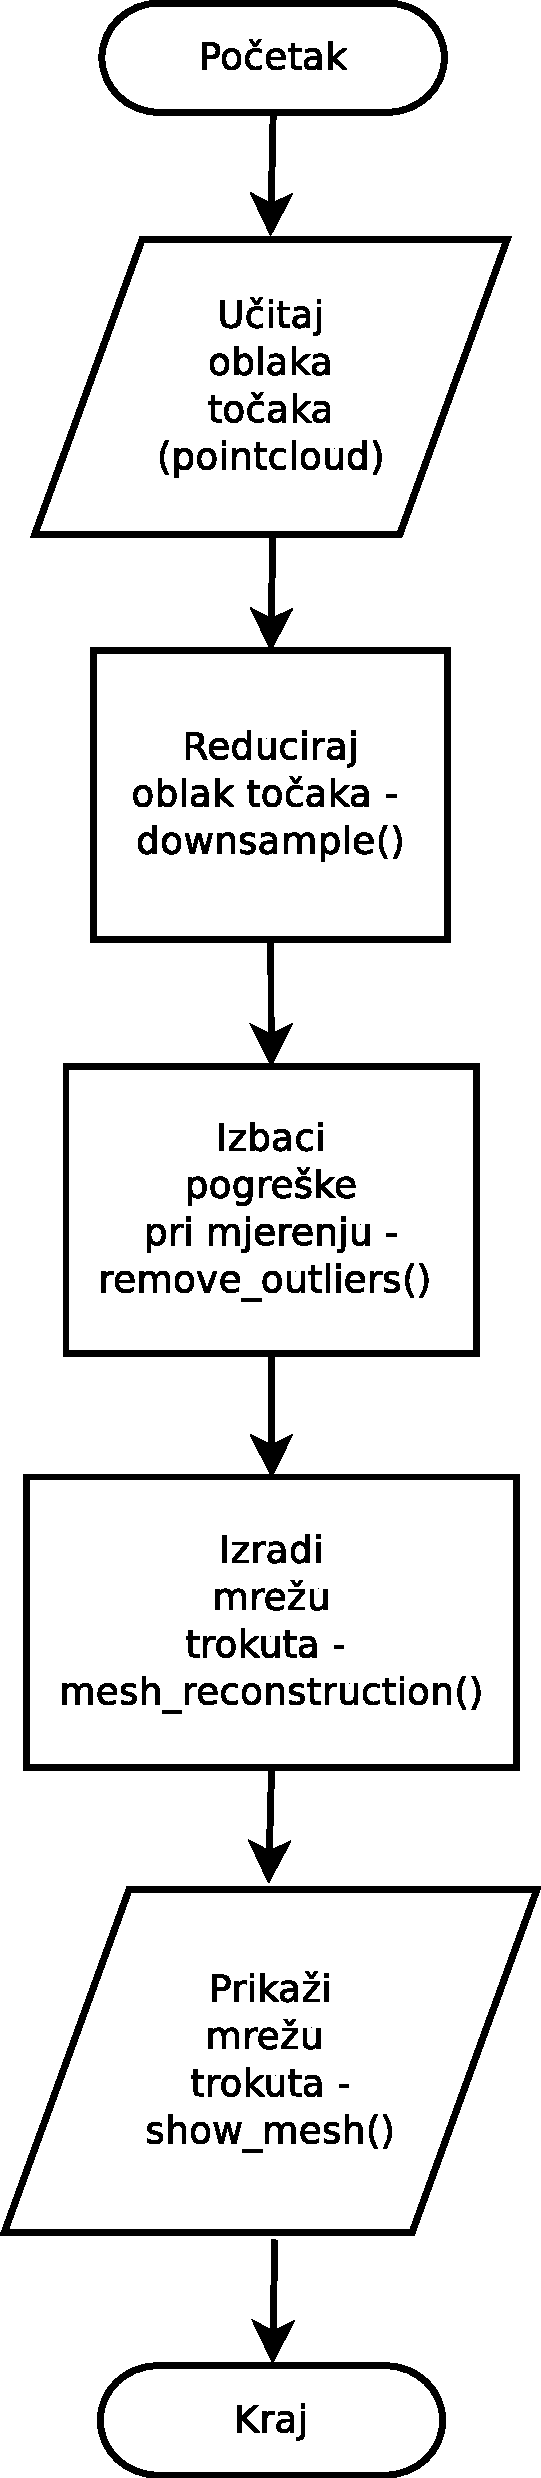
\includegraphics[scale=0.4]{figures/flowchart.pdf}
\caption{Dijagram toka}
\label{fig:{flowchart.pdf}}
\end{figure}

% subsection Izgradnja 3D modela scene pomoću mreže trokuta (end)

% subsection Snimanje scene 3D kamerom i RGBDSlam programom (end)
% section Izgradnja 3D modela scene (end)
